\documentclass[%
10pt, %
final, % 
oneside, % 
onecolumn, %  
centertags]{article} % относится к классу article и размер шрифта 12 пунктовб, {article: статья, report: отчеты и диссертации, book: книга, letter: письмо}

% ------ page construction 

\topmargin= -30pt % насколько сверху будет страница
\textheight= 650pt

% ------ Пакеты расширения

\usepackage[utf8]{inputenc} % задает кодировку, utf-8 кодировка, включающая в себя знаки почти всех языков мира
\usepackage[english, russian]{babel} % подключает необходимые языки, основным языком является английский
\selectlanguage{russian} % настройки будут на английском, но писать будет на русском

\usepackage{euscript}
\usepackage{supertabular}

\usepackage[colorlinks=true,linkcolor=red,unicode=true,urlcolor = blue]{hyperref} %hypered
\usepackage[pdftex]{graphicx} % для графики

\usepackage{amsthm, amssymb, amsmath, amsfonts} % математический пакет, математические шрифты
\usepackage{textcomp}
\usepackage[noend]{algorithmic}
\usepackage[ruled]{algorithm}
\usepackage{lipsum}
\usepackage{indentfirst}
\usepackage{babel}
\usepackage{pgfplots}
\usepackage{setspace}
\usepackage{xcolor}
\usepackage{hyperref}

\linespread{1.2} 
\setlength{\parindent}{2.4em}
\setlength{\parskip}{0.1em}

\pgfplotsset{compat=1.9}
\pgfplotsset{model/.style = {blue, samples = 100}} 
\pgfplotsset{experiment/.style = {red}}

\theoremstyle{plain}
\binoppenalty=10000

\newtheorem{theorem}{Теорема}[section] % theorem

\theoremstyle{definition}
\newtheorem{definition}{Определение}[section]

\theoremstyle{remark}
\newtheorem{remark}{Замечание}[section]

\newtheorem{corollary}{Следствие}

\newtheorem{solution}{Решение}

\newtheorem{proposition}{Proposition}

\newtheorem{example}{Пример}

\newtheorem{lemma}{Лемма}[section]

\renewcommand*{\proofname}{Proof}

\graphicspath{ {./images/} }

\usepackage{fancyhdr}
% % !TEX encoding = UTF-8 Unicode
\usepackage{amssymb, amsmath, natbib, amsthm, graphicx, euscript, mathrsfs, enumerate, empheq}
\renewcommand{\t}[1]{\tau^{(#1)}}
\newcommand{\hgamma}{\hat{\gamma}_{n}}
\newcommand{\bgamma}{\bar{\gamma}_{n}}
\newcommand{\mG}{\mathcal{G}}
\newcommand{\wvn}{\widetilde\varepsilon_{n}}
\newcommand{\A}{\mathscr{A}}
\newcommand{\Par}{\mathscr{P}}
%\newcommand{\eqd}{\stackrel{\mathcal{L}}{=}}
\newcommand{\eqd}{\stackrel{d}{=}}
\newcommand{\lsim}{\lesssim }
\newcommand{\gsim}{\gtrsim }
\newcommand{\corr}{\operatorname{corr}}
\newcommand{\V}{\mathcal{V}}
\newcommand{\BG}{\texttt{BG}}
\newcommand{\PP}{{\mathbb P}}
\newcommand{\Q}{{\mathbb Q}}
\newcommand{\n}{\newline}
\newcommand{\tchi}{\tilde\chi}
\newcommand{\bchi}{\breve\chi}
\newcommand{\bpsi}{\breve\psi}
\newcommand{\bphi}{\breve\phi}
\newcommand{\sign}{\operatorname{sign}}
\newcommand{\diag}{\operatorname{diag}}
\newcommand{\Matr}{\operatorname{Matr}}
\newcommand{\T}{\mathcal{T}}
\newcommand{\E}{{\mathbb E}}
\newcommand{\D}{{\mathbb D}}
\newcommand{\LL}{{\EuScript L}}
\renewcommand{\i}{\mathrm{i}}
\newcommand{\hs}{\hat{s}}
\newcommand{\too}{\rightsquigarrow}
%\def\R{I\!\!R}
%\def\N{I\!\!N}
\newcommand{\Z}{{\mathbb{Z}}}
\newcommand{\N}{{\mathbb{N}}}
\newcommand{\R}{{\mathbb{R}}}
\newcommand{\CC}{{\mathbb{C}}}
\newcommand{\eps}{\varepsilon}
\newcommand{\Ree}{\operatorname{Re}}
\newcommand{\Var}{\operatorname{Var}}
\newcommand{\cov}{\operatorname{cov}}
\newcommand{\supp}{\operatorname{supp}}
\newcommand{\Exp}{\operatorname{Exp}}
\newcommand{\Pois}{\operatorname{Pois}}


\newtheorem{thm}{Теорема}[section]
\newtheorem{lem}[thm]{Лемма}
\newtheorem{cor}[thm]{Следствие}
\newtheorem{prop}[thm]{Утверждение}
\newtheorem{rem}[thm]{Замечание}

\theoremstyle{definition}
\newtheorem{defi}[thm]{Определение}
\newtheorem{ex}[thm]{Пример}

%\renewtheorem{def}{Defition}
%\DeclareMathOperator*{\argmax}{arg\,max}
%\DeclareMathOperator*{\argmin}{arg\,min}
\newcommand{\argmin}{\operatornamewithlimits{arg\,min}}
\newcommand{\argmax}{\operatornamewithlimits{arg\,max}}

\renewcommand{\P}{{\mathbb P}}
\renewcommand{\L}{\mathscr{L}}
\newcommand{\F}{\mathscr{F}}
\newcommand{\dw}{\widetilde{w}}
\newcommand{\bw}{\bar{w}}
\newcommand{\mY}{\mathcal{Y}}
\newcommand{\B}{\mathcal{B}}
\newcommand{\W}{\mathcal{W}}
\newcommand{\vX}{\vec{X}}
\newcommand{\vW}{\vec{W}}
\newcommand{\vu}{\vec{u}}
\newcommand{\vt}{\vec{t}}
\newcommand{\vmu}{\vec{\mu}}
\newcommand{\bd}{\bar{\delta}}
\newcommand{\wY}{\widetilde{Y}}
\renewcommand{\kappa}{\varkappa}
\def\sec#1{\underline{\textbf{#1}}}
\newcommand{\p}{\Upsilon}
\renewcommand{\k}{k}
\renewcommand{\wp}{\widetilde{\p}}
\def\g#1{\bar{g}_{#1}(J)}
\newcommand{\bz}{\breve{\zeta}}
\newcommand{\bp}{\breve{\p}}
\newcommand{\btau}{\breve{\tau}}
\newcommand{\cc}{\breve{c}}
\newcommand{\DD}{\mathcal{D}}
\newcommand{\I}{{\mathbb I}}
\newcommand{\NN}{\EuScript{N}}
\newcommand{\tN}{\widetilde{N}}

\newcommand{\tol}{\xrightarrow{Law}}
\newcommand{\toP}{\xrightarrow{\P}}
\newcommand{\lr}{\leftrightarrow}
\newcommand{\wK}{\gamma}%\widetilde{K}}
\newcommand{\pa}{\partial}

\newcommand{\mm}{s}
\newcommand{\MM}{S}


\pagestyle{fancy}
\fancyhf{}
\lhead{GPN 2020: Data Sciense}
\rhead{Aleksandr Shirokov}

\usepackage{lastpage}

\cfoot{\thepage}

\begin{document}

\begin{titlepage} 
\begin{center}

\textbf{}\\[10.0cm]
\textbf{\LARGE GPN 2020. Data Sciense}\\[0.5cm]
\textsc{\large Выполнил: Александр Широков}

\vfill 

{\large {Solution}} \par
{\large {15.11.2020 г.}} 

\end{center} 
\end{titlepage}

\tableofcontents
\newpage

\section{Input Data}

\subsection{Problem Definition}

В далеком 2148 году мир переживает последствия кризиса и глобальной войны. Постапокалиптическую пустошь населяют безжалостные воины, но все еще есть место для честных предпринимателей.  

Вы работаете в Компании, управляющей сетью магазинов, которая торгует различными товарами, пользующимися спросом в данной реальности.

Вам доступны исторические данные о продажах за 2 года и данные о характеристиках магазинов.

\textbf{Problem}:

Для лучшего управления магазинами, в частности, для более оптимального планирования промо-кампаний и прогнозирования спроса, вам необходимо \textbf{разбить магазины на кластеры похожих}. Единственный способ, которым пользовалась компания в прошлом – это разбитие по географическому признаку, то есть по городам. Но вы верите, что прочие характеристики магазинов, а самое главное, профили продаж магазинов, помогут сделать это гораздо точнее.

Вы должны изучить данные, выбрать метрику качества кластеризации, придумать и посчитать информативные признаки (например, доля продаж «патронов» по пятницам) и построить наиболее качественный алгоритм кластеризации, а также описать смысл каждого кластера в понятном для управляющих вашей Компании виде.

С этого момента начается моё слово.

\subsection{Table \textit{sales}}

Таблица \textit{sales} содержала $5081459$ записей по продажам за $2$ года с \textsc{01.01.2146} по  \textsc{01.01.2148}

\begin{center}
	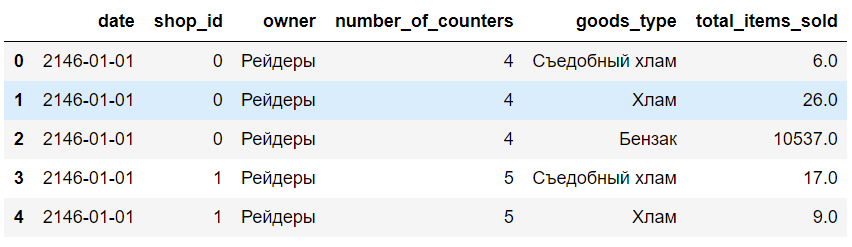
\includegraphics[scale=0.35]{1.png}

 	Рис.1 Таблица \textit{sales}
\end{center}

cо следующими признаками:
\begin{itemize}
	\item \textsc{date} - дата продажи товара $Y-M-d$	
	\item \textsc{shop\_id} - уникальный идентификатор магазина: в интервале $[0, 844]$, \textsc{integer}
	\item \textsc{owner} - владелец магазина, строковый тип, $5$ уникальных владельцев: 
	\begin{enumerate}
		\item Рейдеры - $3906481$ - самая многочисленная группа
		\item Воины полураспада - $595022$
		\item Стервятники - $275076$
		\item Последователи Апокалипсиса - $169120$
		\item Бомбисты - $135760$
	\end{enumerate}
	\item \textsc{number\_of\_counters} - количество работающих прилавков/продавцов, \textsc{integer}
	\item \textsc{goods\_type} - тип товара, всего $11$ видов товара, string
	\item \textsc{total\_items\_sold} - суммарные продажи в этот день в магазине в штуках, \textsc{float}
\end{itemize}

В таблице отсутствовали пропущенные значения. Проведём некий разведывательный анализ данной таблицы. Для начала я сгенерировал новые признаки:
\begin{itemize}
	\item \textsc{year} - год продажи: $[2146, 2147]$
	\item \textsc{month} - месяц продажи: $[1, \ldots, 12]$
	\item \textsc{day} - день продажи: $[1, 31]$
	\item \textsc{doy} - номер дня в году: $[1, 365]$
	\item \textsc{day\_name} - название дня недели: \textsc{Monday, ..., Saturday}
	\item \textsc{month\_name} - название месяца: \textsc{January, ..., December}
	\item \textsc{is\_weekend} - является ли день выходным днём: $[0, 1]$
\end{itemize}

Для чего я вообще начал проводить разведывательный анализ. Идея моя заключалась в следующем: для кластеризации на некоторые группы магазинов хотелось бы найти такие признаки, по которым наши магазины имели какие-то различия в продажах, количестве продавцов и.т.д. Для этого я и начала получать описательные статистики в некоторых разрезах. Вот некоторые результаты, которые удалось получить:
\begin{itemize}
	\item Среднее количество продаж по месяцам в разрезе \textsc{shop\_id} не выявило никаких явных различий - всегда получалось распределение по типу Пуассоновского, но с очень тяжёлыми хвостами. Такая же картина и в разрезе по годам - картина абсолютно идентичная
	\begin{center}
	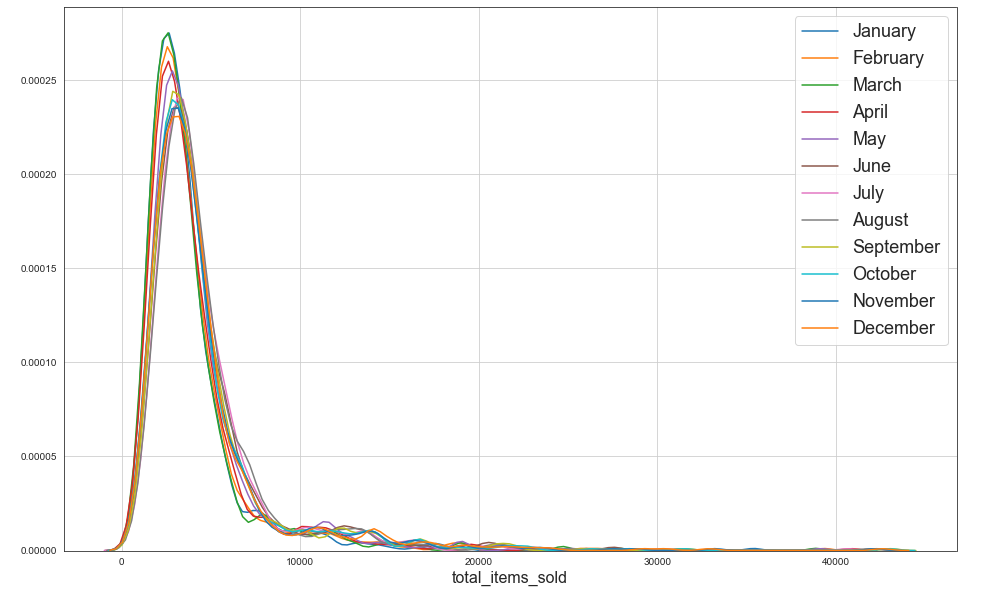
\includegraphics[scale=0.35]{2.png}

 	Рис.2 Распределение гистограмма средних продаж по магазинам в разрезе по дням недели и виду товара
 	\end{center}
 	\item При анализе среднего количества проданных товаров было выяснено, что самыми продаваемыми товарами являются \textsc{Бензак} и \textsc{Солярка}, стягивающие на себя в основном все продажи.
	\begin{center}
	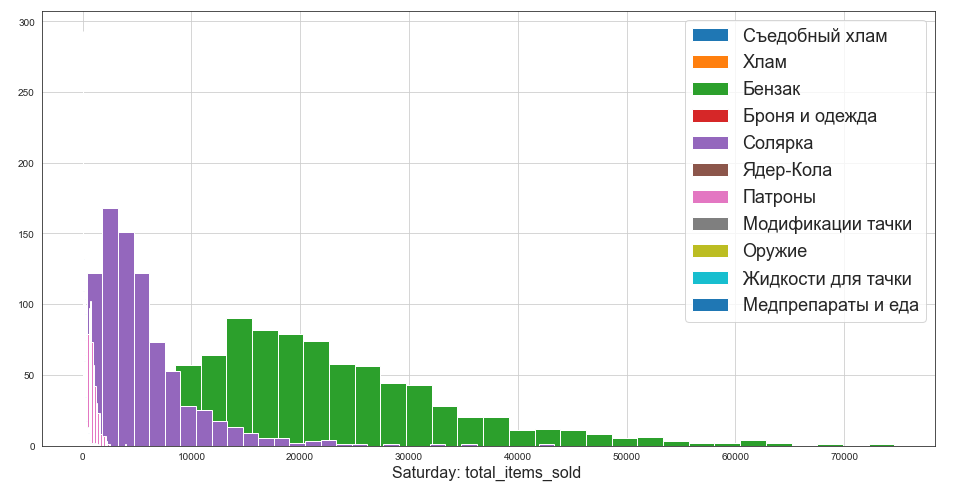
\includegraphics[scale=0.35]{3.png}

 	Рис.3 Распределение гистограмма средних продаж по магазинам в разрезе по товарам
 	\end{center}
 	Тем не менее вид товара не влияет на распределение продаж в разрезе по дням недели - данная картина наблюдается для каждого дня недели.
 	\begin{center}
	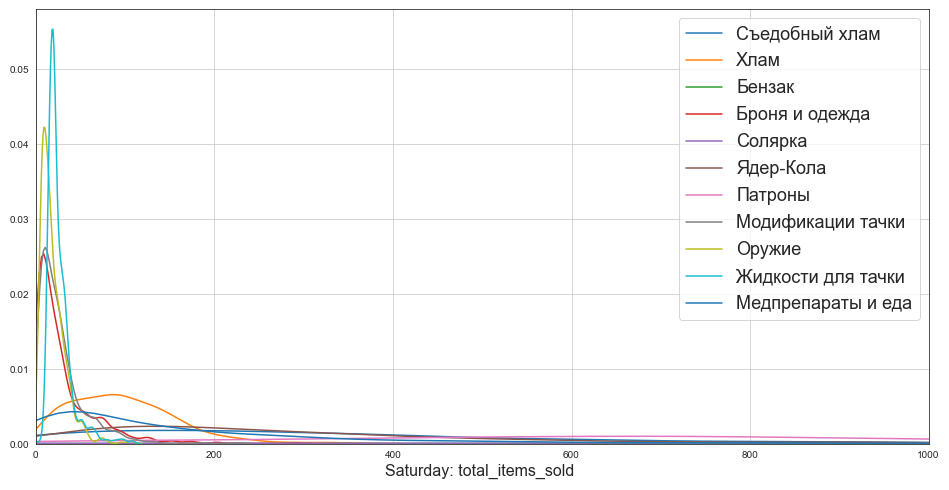
\includegraphics[scale=0.35]{4.png}

 	Рис.4 Распределение гистограмма средних продаж по магазинам в разрезе по дням недели (суббота)
 	\end{center}
 	Зато если взять общее распределение, то видно, что в пятницу суммарные продажи товаров являются наименьшими, а в среду - наибольшими. Средие суммарные продажи приходятся на понедельник.
 	\begin{center}
	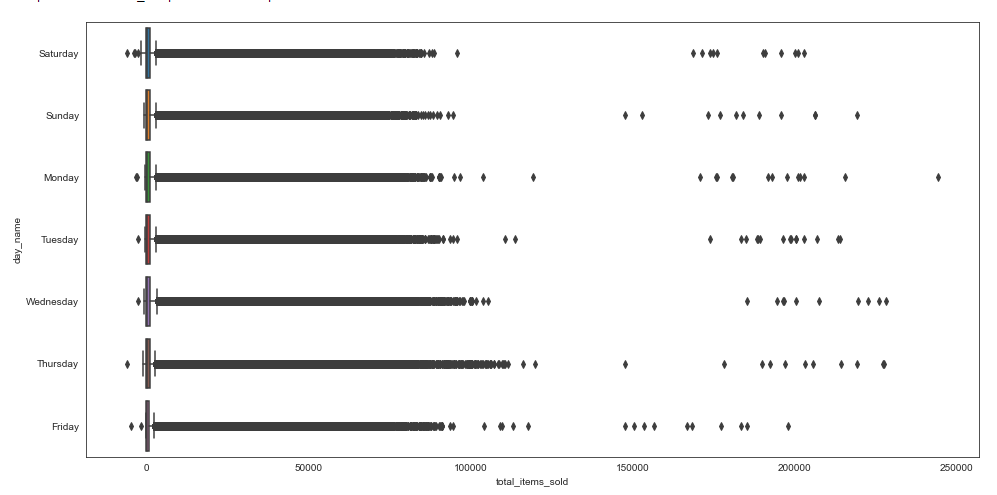
\includegraphics[scale=0.35]{5.png}

 	Рис.5 Суммарные продажи в магазинах в разрезе по дням недели
 	\end{center}
 	\item Проводился так же анализ средних продаж в разрезе по владельцам магазинов - \textsc{owner}.
 	\begin{center}\label{formula2}

	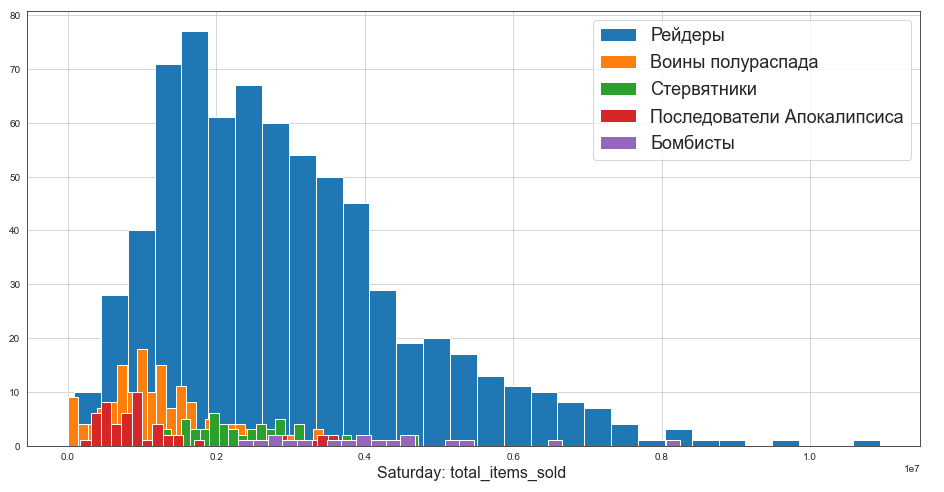
\includegraphics[scale=0.35]{6.png}

 	Рис.6 Суммарные продажи в магазинах в разрезе по владельцам магазинов
	\end{center}
 	Видно, что наибольшие продажи на себя стягивают "Рейдеры" (синие), затем "Воины полураспада" (оранжевые) и затем идёт группа из самых маленьких продаж. На самом деле, уже на этом были мысли по поводу кластеризации: если есть какая-то гистограмма плотности распределений, то кластеризацию вполне можно проводить на основании данной плотности, наблюдая за количество горбов в гистограмме. Да и из картинки напрашивается распределение магазинов на "продающих много", "продающих средне" и продающих "очень мало". Но ведь неоходимо понять, из-за чего магазины получают преимущество над другими магизинами.

 	Немного отвлечемся и посмотрим на разницу в распределениях для продаж товара "Бензак" и "Броня и одежда" в разрезе по владельцам:
 	\begin{center}
	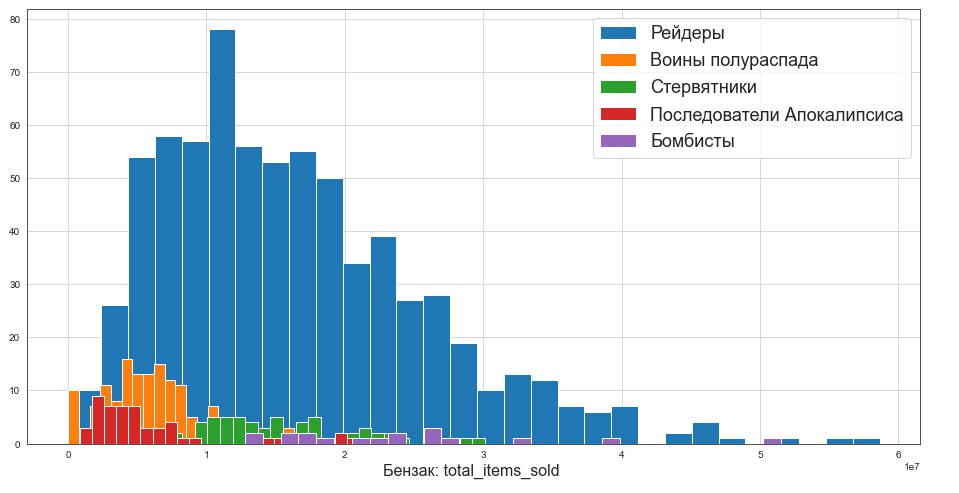
\includegraphics[scale=0.35]{7.png}

 	Рис. 7 Продажа товара "Бензак" - нет явного перекоса в нулевой столбец на гистограмме
	\end{center}
	\begin{center}
	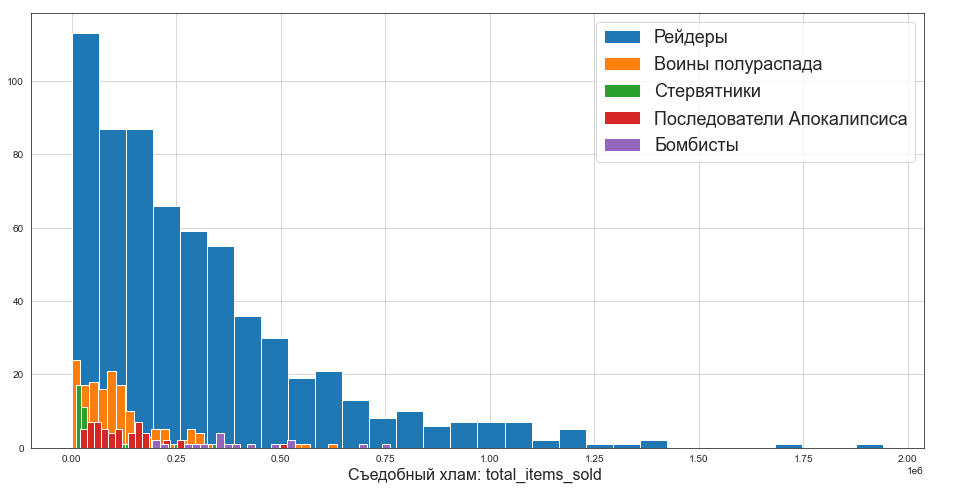
\includegraphics[scale=0.35]{8.png}

 	Рис. 8 Видно, что есть нулевой столбик явно выделяющийся на гистограммах - так выглядят все гистограммы для непродающихся товаров
	\end{center}
	\item Далее я посмотрел на количество продавцов и поинтересовался: менялось ли количество продавцов координально с течением времени. Это вопрос даст нам ответ про стабильность ситуации в нашем апокалиптическом обществе. 
	\begin{center}
	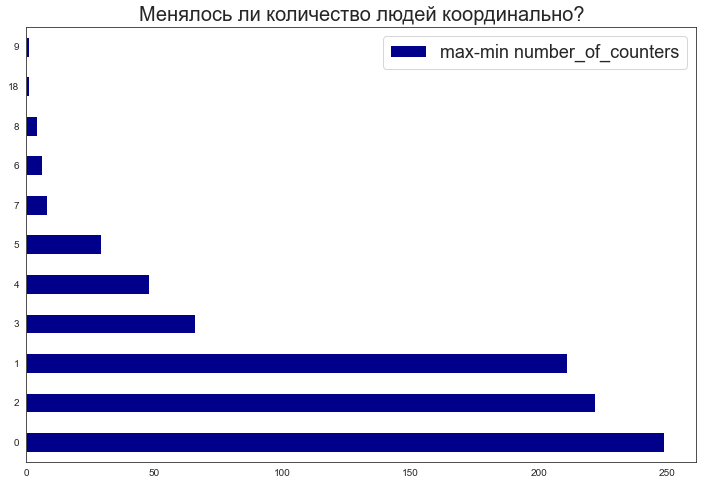
\includegraphics[scale=0.35]{9.png}

 	Рис. 9 Разница между максимальным значением продавцов и минимальным в течение времени
	\end{center}

	Видно, что количество продавцов практически не менялось ($\pm 2$). Было только несколько случаев, когда кто-то из владельцев "психанул" и добавил $18$ новых продавцов. Видимо, хотел улучшить продажи. В качестве вывода можно сказать, что по данном фактора кластеризация не будет происходить.
	\item Распределение продаж по будням и на выходных:
	\begin{center}
	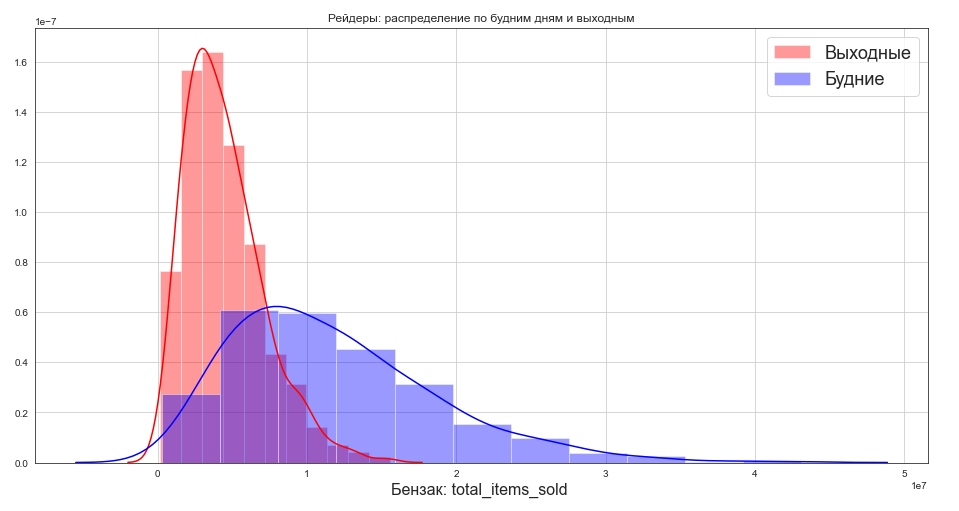
\includegraphics[scale=0.35]{10.png}

 	Рис. 10 Суммарные продажи по будням и на выходных
	\end{center}

	По выходным суммарное значение выручки больше, чем по будням, но как мы видим - с очень маленькими хвостами, а по будням - среднее значение выручки меньше, но хвосты тяжелые, поэтому логично предположить, что плотность распределения средних значений будет примерно одинаковая.

	\begin{center}
	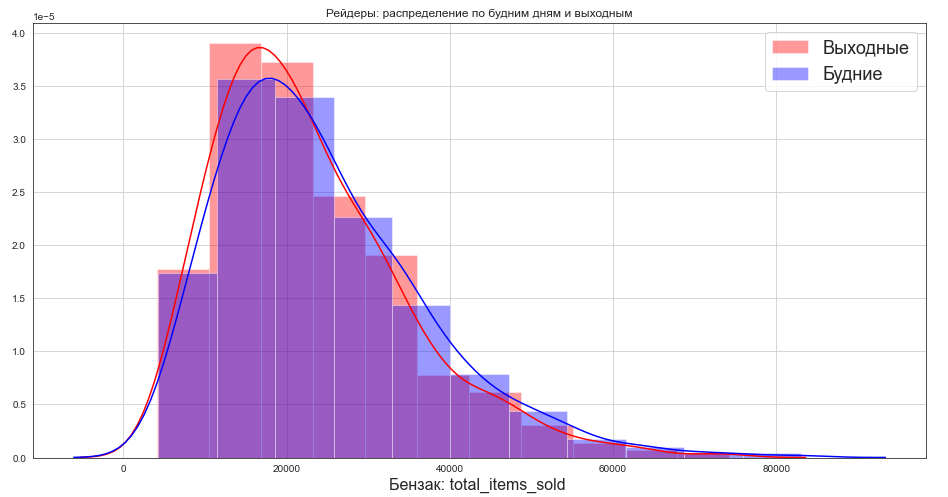
\includegraphics[scale=0.35]{11.png}

 	Рис. 11 Средние продажи по будням и на выходных. Как и было предположено
	\end{center}

	Различий в гистограммах в разрезе по дням недели и товарам не были выявлены.
\end{itemize}

\textbf{Выводы из таблицы} \textit{sales}: были выявлены различия в распределених продаж товара "Бензак" и "Солярка" в сравнении с другими товарами, было выявлено, что по пятницам товары продаются меньше всего на недели, а в среду - больше всего, а так же магазины подразделяются на три категории в разрезе по владельцам магазинов: большие, средние и очень маленькие продажи. Перейдем к рассмотрению таблицы \textit{cities}.

\subsection{Table \textit{cities}}

В таблице \textit{cities} представлена информация о принадлежности города определенному местоположению - \textsc{location}. Всего региона $3$: \textsc{Скалистый Могильник, Свистящие Степи и Радиоактивная Пустошь}и города распределены равномерно по данным регионам: $6, 4, 4$ соответственно. Более информации нет, поэтому перейдем к таблице \textit{shops}.


\subsection{Table \textit{shops}}

Данная таблица содержит информацию по характеристикам магазинов и не зря сказано в описании, что данная таблица является менее точной, так как ведётся вручную - уже с самого начала я ожидал трудности с заполнением пропущенных данных. 

Таблица \textit{shops} содержала $845$ записей с характеристиками магазинов cо следующими признаками:

\begin{itemize}
	\item \textsc{shop\_id} - PK, уникальный идентификатор магазина: $[0, \ldots, 844]$
	\item \textsc{neighborhood} - в какой окрестности находится магазин, категориальный признак, имеется $7$ уникальных значений, без пропущенных: \textsc{В центре, Промзона, У ночлега, У воды, На отшибе, У тоннеля< С краю}
	\item \textsc{city} - в каком городе открыт магазин, категориальный признак.

	На данном этапе хочется остановиться, потому что именно в этом признаке скрывается \textbf{причина неудчаной кластеризации по городам}. Если просмотреть на частоту встречаемости городов, то увидим следующее:
	\begin{center}
	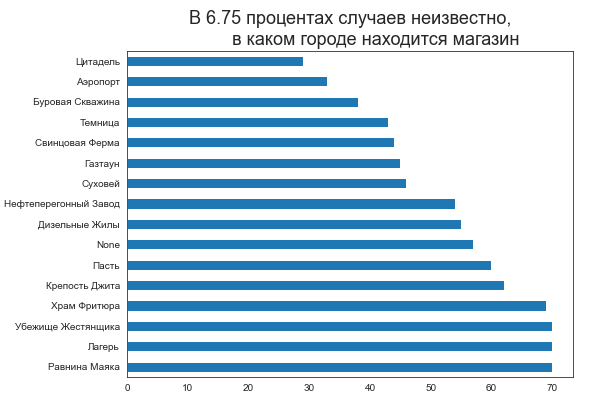
\includegraphics[scale=0.5]{12.png}

 	Рис. 12 Встречаемость определённых городов в таблице \textit{sales}
	\end{center}

	Видно, что в практические $7\%$ случаев неизвестно (\textsc{None}), в каком городе находится магазин. В этом и есть причина, по которому кластеризация по городам не является оптимальным - во-первых, у нас много городов и большое количество кластеров.. весьма неинтерпретируемо, во-вторых у нас весьма велика вероятность (она сравнима с вероятностями других городов) того, что какой-то магазин мы просто не сможем обнаружить в этом столбце и примерно 7 столбцов наблюдений мы просто выкидываем. А вдруг данный \textsc{shop\_id} принадлежит "Рейдерам" и мы потеряем огромное количество прибыли из рассмотрения (такое же возможно). Поэтому, кластеризация по городам - не очень хорошая идея, постараемся придумать получше, получается. Да и что делать с пропущенными значениями - не особо понятно. Было принято решение не включать данный категориальный признак в общее рассмотрение, раз кластеризация не будет проводиться по нему.
	\item \textsc{year\_opened} - в каком году был открыт магазин. В $63$ случаях (второе место по встречаемости) неизвестно было в каком году был открыт магазин, поэтому было предпринято следующее преобразование данного признака: отсутствующие значение заменим на \textit{медиану} по столбцу, а дальше каждое значение заменим на разность $2147 - X$, где $X$ - значение года открытия. Таким образом мы переходим к некоторой описательной статистики открытия города.
	\item \textsc{is\_on\_the\_road} - находится ли магазин прямо у дороги. Распределение значений следующее: нет - $614$, да - $224$ и в $7$ случаях неизвестно. Данный категориальный признак можно прокодировать с помощью \textsc{OneHotEncoding}, а пропущенные значения заменить на самое встречаемое значение - $0$.
	\item \textsc{is\_with\_the\_well} - есть ли у магазина колодец. У данного признака есть явный перекос в сторону "нет" - не имеет, поэтому было принято решение не применять кодирование - был бы очень сильный дисбаланс.
	\item \textsc{is\_with\_additional\_services} - есть ли в магазине дополнительные сервисы. Данный признак является сбалансированным, по половине наблюдений за "нет" и "да".
	\item \textsc{shop\_type} - тип магазина, всего $4$ типа. И на самом деле я изначально ставил очень много надежд на этот признак и вот в чём дело. У данного признака есть много пропущенных значений - примерно пятая часть. И если бы по данному признаку можно было бы кластеризировать магазины, то задача переформуровалась в задачу обучения с учителем - есть $4$ класса и необходимо предсказать для отсутсвующих классов принадлежность определённому классу. Эта задача была бы намного приятнее. Были предприняты попытки генерирования признаков и на основании алгоритма $K$-ближайших соседей собственной реализации (из прошлых времен) предсказывать классы - по виду магазина. Но, к сожалению, данный признак не показал различий в распределениях продаж товаров, продаж по владельцам магазинов и.т.д. Но переход к задаче обучения с учителем на основании какого-то признака - та идея, которую следует иметь ввиду и я бы в эту сторону хорошенько подумал.
\end{itemize}

Из некоторых выводов: мы заполнили пропущенные значения< отбросили несбалансированные признаки и предложил несколько идей для кластеризации. Так же было сделано наблюдение, что если в одном из последних $6$ признаков отсутствовало значение, то, в принципе информация о данном магазине отсутстовала и данные можно удалить из таблицы для упрощения кластеризации. 

Осталось рассмотреть общую \textsc{Merge} таблицу. 

\subsection{Table Merge: \textit{sales | shops | cities}}

Соединим сначала таблицы \textit{shops} и \textit{sales} по столбцу \textsc{city}, а затем полученную таблицу соединим по столбцу \textsc{shop\_id} с таблицей \textit{sales}.

Проведём опять анализ данной таблицы. 

\begin{itemize}
	\item Для начала хотелось бы понять, какое местоположение является наиболее выгодным: для этого будем использовать данные о суммарных продажах по магазинам в разрезе по столбцам \textsc{owner} и \textsc{neighborhood}. Для того, чтобы получить информацию о наилучшем местоположении, я провёл следующий алгоритм: брал магазины с владельцем \textsc{owner} и сопоставлял самому большому значению выручки в разрезе по \textsc{neighborhood} минимальный ранг и.т.д. В итоге так сделал для всех owner и посчитал сумму рангов. В итоге получились следующие результаты:
	\begin{enumerate}
		\item \textsc{В центре} - наиболее выгодное местоположение, сумма рангов - $0$.
		\item \textsc{У тоннеля, С краю} - делят 2/3 места, сумма рангов - $9$
		\item \textsc{Промзона} - суммар рангов - $13$
		\item \textsc{У ночлега} - суммар рангов - $16$
		\item \textsc{На отшибе} - суммар рангов - $20$
		\item \textsc{У воды} - суммар рангов - $21$
	\end{enumerate}

	Мы нашли признак, по которому распределения разные выручки. Возьмём на вооружение..
	\item Далее я попытался проверить теорию о кластеризации по \textsc{shop\_id}, но пришло разочарование:
	\begin{center}
	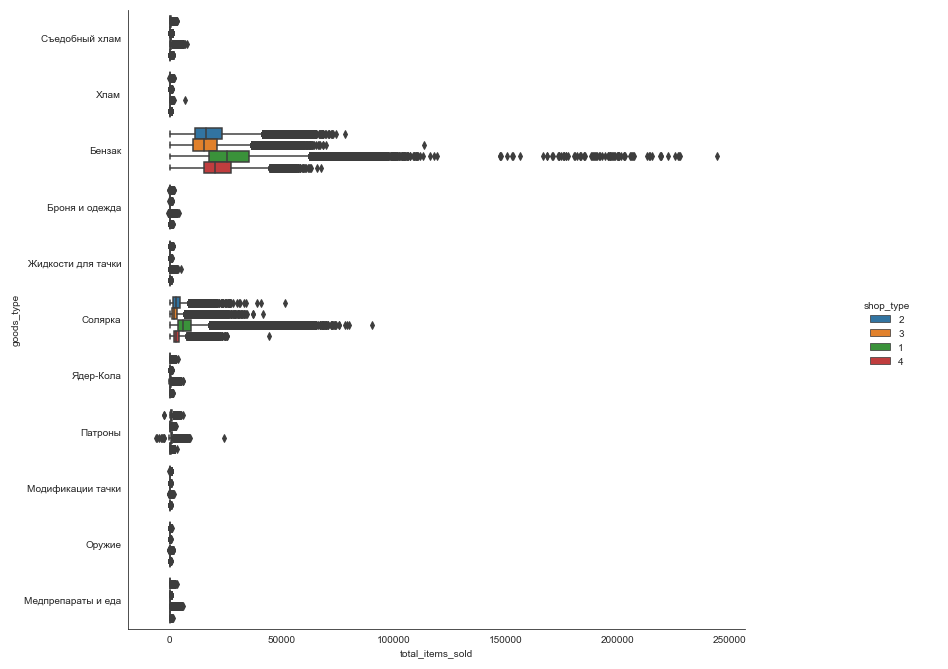
\includegraphics[scale=0.4]{13.png}

 	Рис. 13 Разрез по \textsc{shop\_id} в зависимости от продажи товаров
	\end{center}
	\begin{center}
	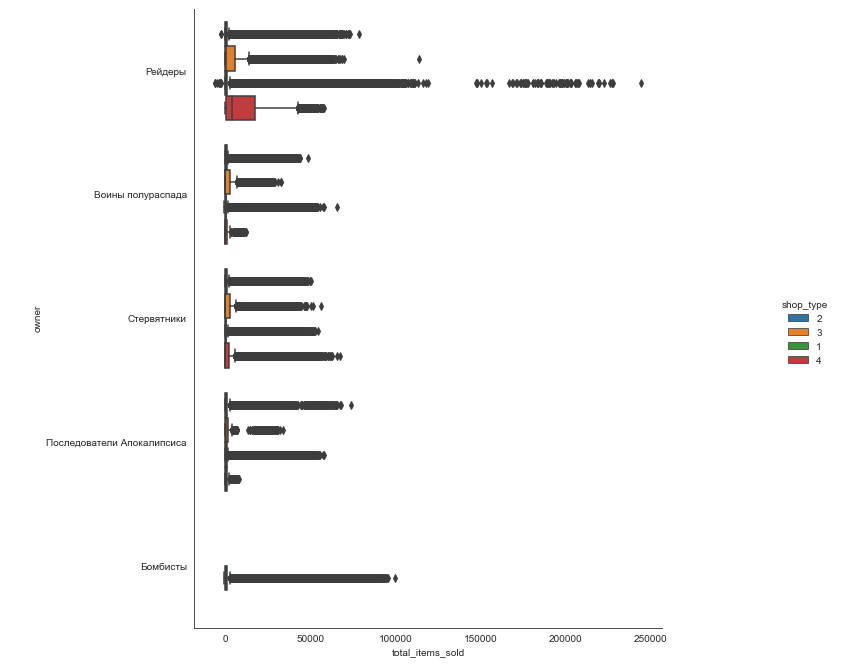
\includegraphics[scale=0.4]{14.png}

 	Рис. 14 Разрез по \textsc{shop\_id} в зависимости от владельца
	\end{center}

	Видно, что распределения одинаковы в разрезах по товарам одинаковое, а вот второй рисунок.. Он оставляет надежду на кластеризацию по данному признаку, но я просто побоялся, если честно, его интерпретировать, потому что по идее можно здесь разбить на $3$ класса, но бомбисты уж очень явно различаются... В общем идею с применением обучения с учителем по предсказанию пропущенных значений в \textsc{shop\_id} я отложил и не притронулся больше.
	\item Теперь проанализируем, есть ли различия при наличии дороги
	\begin{center}
	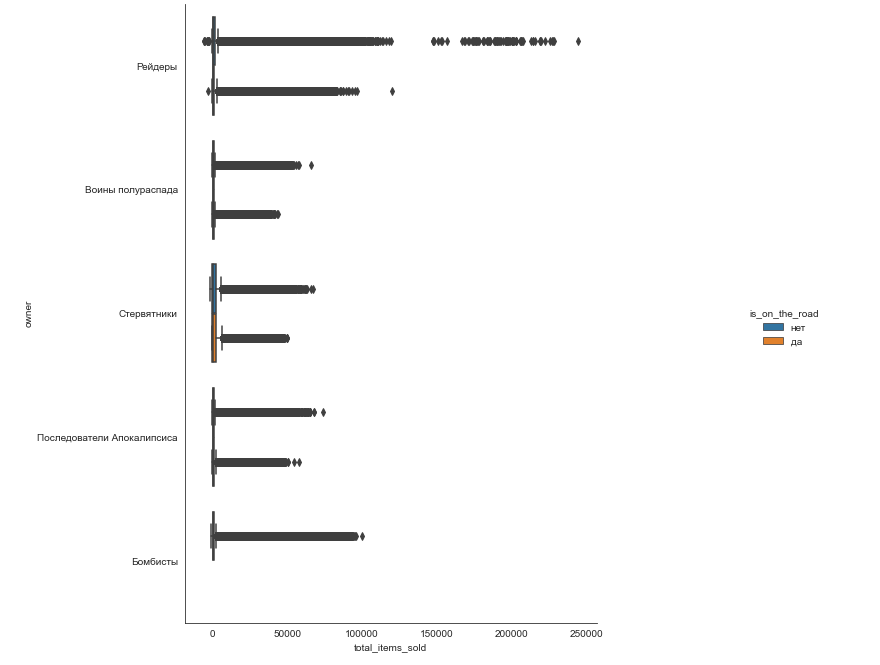
\includegraphics[scale=0.4]{15.png}

 	Рис. 15 Видим, что лучше продаются магазины не находящиеся рядом с дорогой.
	\end{center}
	
	\item Проанализировав признак \textsc{is\_with\_the\_well} было выяснено, что распределения не зависят от наличия или отсутствия данного признака - удалим из рассмотрения.
	\item  \textsc{is\_with\_additional\_services}
	\begin{center}
	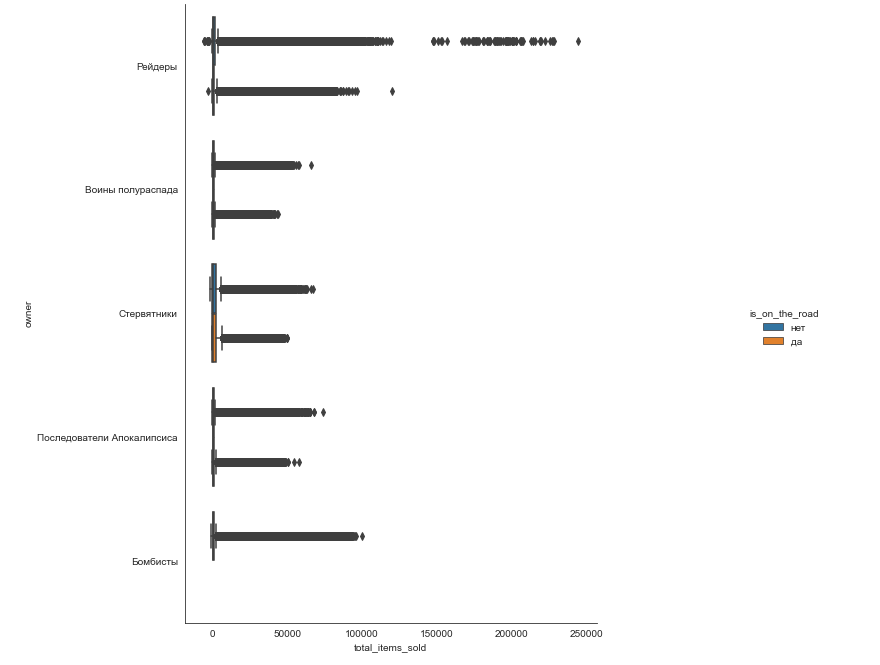
\includegraphics[scale=0.4]{15.png}

 	Рис. 16 Видим, что у "Стервятников" продажи больше при наличии дополнительных сервисов
	\end{center}
\end{itemize}

Некоторые выводы: мы подходим к важному этапу: построение гипотезы кластеризации. Действуя по изначально намеченному плану, мы искали признаки, на основании которых распределения тех или иных статистик различались. Перейдем к построению гипотезы кластеризации:

\subsection{Hypothesis of Clusterisation}

На данном этапе появилася \textbf{гипотеза кластеризации}: будем кластеризировать магазины по выгодности местоположения, откуда следует принадлежность определённому кластеру: маленькой, средней или большой компании, а так же, чем выгоднее местоположение, тем больше выручка с основных товаров, которые продаются в магазинах: \textsc{Солярка}, \textsc{Бензак}.

Это гипотеза звучит логично: разделим наши магазины на несколько групп по выгодности местоположения (у реки или в центре - разница есть), а из выгодности местоположения делается вывод о том, какая компания могла бы выкупить выгодное местоположение - очевидно, что богатая. Из выгодности местоположения вытекает увеличиние выручки.

Перейдем к генерации признаков и кластеризации.

\newpage
\section{Clustersisation}

\subsection{Feature Engineering}

Создадим матрицу признаков, на основании которых мы будем делать кластеризацию. Идея следующая сгенерируем признаки таким образом, чтобы по тем признакам из первой части моего отчёта, где наблюдались различия в распределениях, мы взяли самые плохо продаваемые категории, средние и наиболее хорошо продаваемые. Из этого метода сгенерируем следующую матрицу признаков, состоящую из:
\begin{itemize}
	\item - среднее количество \textsc{total\_items\_sold} по продуктам "Бензак", "Оружие", "Хлам" и "Броня и Одежда" - будем придерживаться данной стратегии - выбирать наилучшее по продажам среднее и наихудшее. После каждого добавления заполняем нулевые значения минус максимальным значеним в "dataframe", чтобы обозначить различие между возникающими классами более явно.
	\item среднее количество по дню \textsc{dat\_name} недели: Пятница, как наименьшее, Thursday - как наибольшее и \textsc{Monday} - как нечто среднее.
	\item количество продаж по наличию или отсутствию дополнительных сервисов
	\item среднее количество продаж по владельцам "Рейдеры" и "Бомбисты"
\end{itemize}

\subsection{Use Metric: \textit{Silhouette}}

Будем использовать метрику \textsc{silhouette} для оценки качества кластеризации.

Для одного элемента $x$ она считается так:
$$S(x) = \frac{b(x) - a(x)}{\max{(a(x), b(x))}}$$
где
\begin{itemize}
 	\item $a(x) =$ среднее расстояние от x до точек внутри того же кластера.
 	\item $b(x) = $ среднее расстояние от x до точек внутри ближайшего кластера.
\end{itemize} 

Сама метрика равна среднему значению $S(x)$ от каждого элемента.

Видно, что $-1 \leqslant S(x) \leqslant 1$, причем чем больше $b(x)$ относительно $a(x)$, тем метрика ближе к $1$. Чем метрика больше - тем лучше кластеризация.

\subsection{Use Method: Agglomerative Clustering}

Будем использовать алгоритм \textsc{Agglomerative Clustering}. Интуиция у алгоритма простая:
\begin{enumerate}
	\item Начинаем с того, что высыпаем на каждую точку свой кластер
	\item Сортируем попарные расстояния между центрами кластеров по возрастанию
	\item Берём пару ближайших кластеров, склеиваем их в один и пересчитываем центр кластера
	\item Повторяем п. 2 и 3 до тех пор, пока все данные не склеятся в один кластер
\end{enumerate}

Применим алгоритм \textsc{AgglomerativeClustering} к нашим признакам.

\subsection{Clusterisation: Result}
\begin{center}
	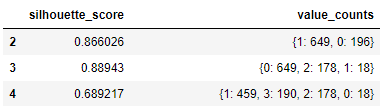
\includegraphics[scale=0.6]{17.png}

 	Рис. 17 Результаты кластеризации \textsc{AgglomerativeClustering} по метрике \textsc{Silhouette}
	\end{center}

По результатам кластеризации можно сделать вывод, что при $k=3$ у нас наибольшее значение метрики, но самое главное - этот результат весьма предсказуем - мы разделили наше множество на $3$ магазина, причём второй и первый класс, как видно из результатов, весьма похожи друг на друга, а это именно то, о чём мы говорили, когда предполагали, что кластеризовать можно по большим, средним и маленьким компаниям (страница \pageref{formula2}). Так же выяснено, что полученные кластеры получились, если принять во внимание местоположение магазина, то есть выручка зависит от выгодности местоположения магазина.

Характеристики полученных кластеров:
\begin{itemize}
	\item Класс №0 ($649$) - наиболее представимый класс, большинство из магазинов принадлежат двум самым богатым продавцам, так же практически все данные магазины имеют наибольшую среднюю выручку и магазины располагаются в большинстве своём 'В центре' либо 'У тоннеля', не имеет различий в том, есть ли дополнительные сервисы или нет
	\item Класс №1 ($178$) - очень сильно проигрывает классу №0, имеет намного меньшую среднюю выручку, расположены в в остальных участках \textsc{neighborhood}, но имеют различия в выручке при наличии дополнительных сервисов в большую сторону
	\item Класс №2 ($18$) - во многом очень схожий с классом №1, имеет схожую выручку, но местоположение - у Воды (в большинстве своём) и выручка не зависит от наличия дополнительных сервисов
\end{itemize}

Результаты кластеризации были загружены в файл \textbf{\textsc{submission.tsv}}
\newpage

\section{Conclusion}

Построенный алгоритм качественно проводит кластеризацию на данных объектах и имеет понятную интерпретацию, но по сути мы кластеризуем наши данные на основании количества продаж и (слава богу) сумели найти признак различия выгодности местоположений, что, однако, является не причиной, а следствием основного нашего признака. Поэтому, я бы попросил информацию о количестве людей, находящихся в магазине каждый день, о популяции городов (например), добавил бы некоторого разнообразия в данные, хотя и на доступных нам данных мы смогли вытянуть очень много информации, как мне кажется.

Мне понравилось заниматься данной задачей и мне бы хотелось продолжить ею заниматься, потому что я, конечно, чувствую, что загадка этой задачи не раскрыта и наполовину, но я не ограничился одни лишь предложением данной кластеризации: в отчёте я предлагал несколько идей, в направлении которых можно двигаться в дальнейшем. 

В \textsc{solution.ipynb} находится оформленный \textsc{jupyter notebook} с выводами и реализованной кластеризацией.

Спасибо за задание! Мне было интересно решать и, я надеюсь, что на данном этапе мы не остановимся.

С Уважением, Александр Широков
\end{document}

